\chapter{Introduction}
\label{chapter:Introduction}
%\epigraph{Saving our planet, lifting people out of poverty, advancing economic growth... these are one and the same fight. We must connect the dots between climate change, water scarcity, energy shortages, global health, food security and women's empowerment. Solutions to one problem must be solutions for all.}{\textit{Ban Ki-moon}}

%This dissertation considers a way to solve the global problems of energy shortage and environment problem.

\section{Research background and significance}
% 现有太阳能光热发电技术简析,提出太阳能梯级发电的背景及其意义。

% 能源和环境现状
%REN21, a global renewable energy policy multi-stakeholder network, published the most comprehensive annual overview of renewable energy of 2016.~\cite{REN21}
Renewables are now established around the world as mainstream sources of energy. Rapid growth, particularly in the power sector, is driven by several factors, including the improving cost-competitiveness of renewable technologies, dedicated policy initiatives, better access to financing, energy security and environmental concerns, growing demand for energy in developing and emerging economies, and the need for access to modern energy.
%An estimated 147 gigawatts (GW) of renewable power capacity was added in 2015.

% 太阳能光热发电现状
Solar energy, which has the advantages of widely distribution, huge amount, inexhaustible and no pollution, has received much attention by many countries and been regarded as the best potential candidate of the fossil energy. The International Energy Agency projected in 2014 that under its ``high renewables'' scenario, by 2050, solar photovoltaics and concentrating solar thermal power would contribute about 16 and 11 percent, respectively, of the worldwide electricity consumption, and solar would be the world's largest source of electricity.~\cite{IEA2014}

Concentrating solar thermal power generation is another form of power generation technology except solar photovoltaic power generation. Concentrating Solar Power (CSP) system uses mirrors to converge sunlight onto a receiver that absorbs the solar energy and transfer it to a heat transfer fluid (HTF) such as a synthetic oil, molten salt or air. The HTF then directly or indirectly used as the heat source in a power cycle.
Compared to solar photovoltaic, solar thermal power is gaining more attention for its advantages as higher energy density, smooth power generation, good grid compatibility, easy to integrate with existing fossil power plant.

% 文献1
Concentrating solar power technologies use different mirror configurations to concentrate the sun's light energy onto a receiver and convert it into heat. The heat is collected for power generation or used as industrial process heat.
There are three types of CSP technologies being commercially applied: parabolic trough, parabolic dish and power tower.
Figure~\ref{fig:collectors} shows examples of the three types of CSP technologies.
\begin{figure}[!ht]
\centering
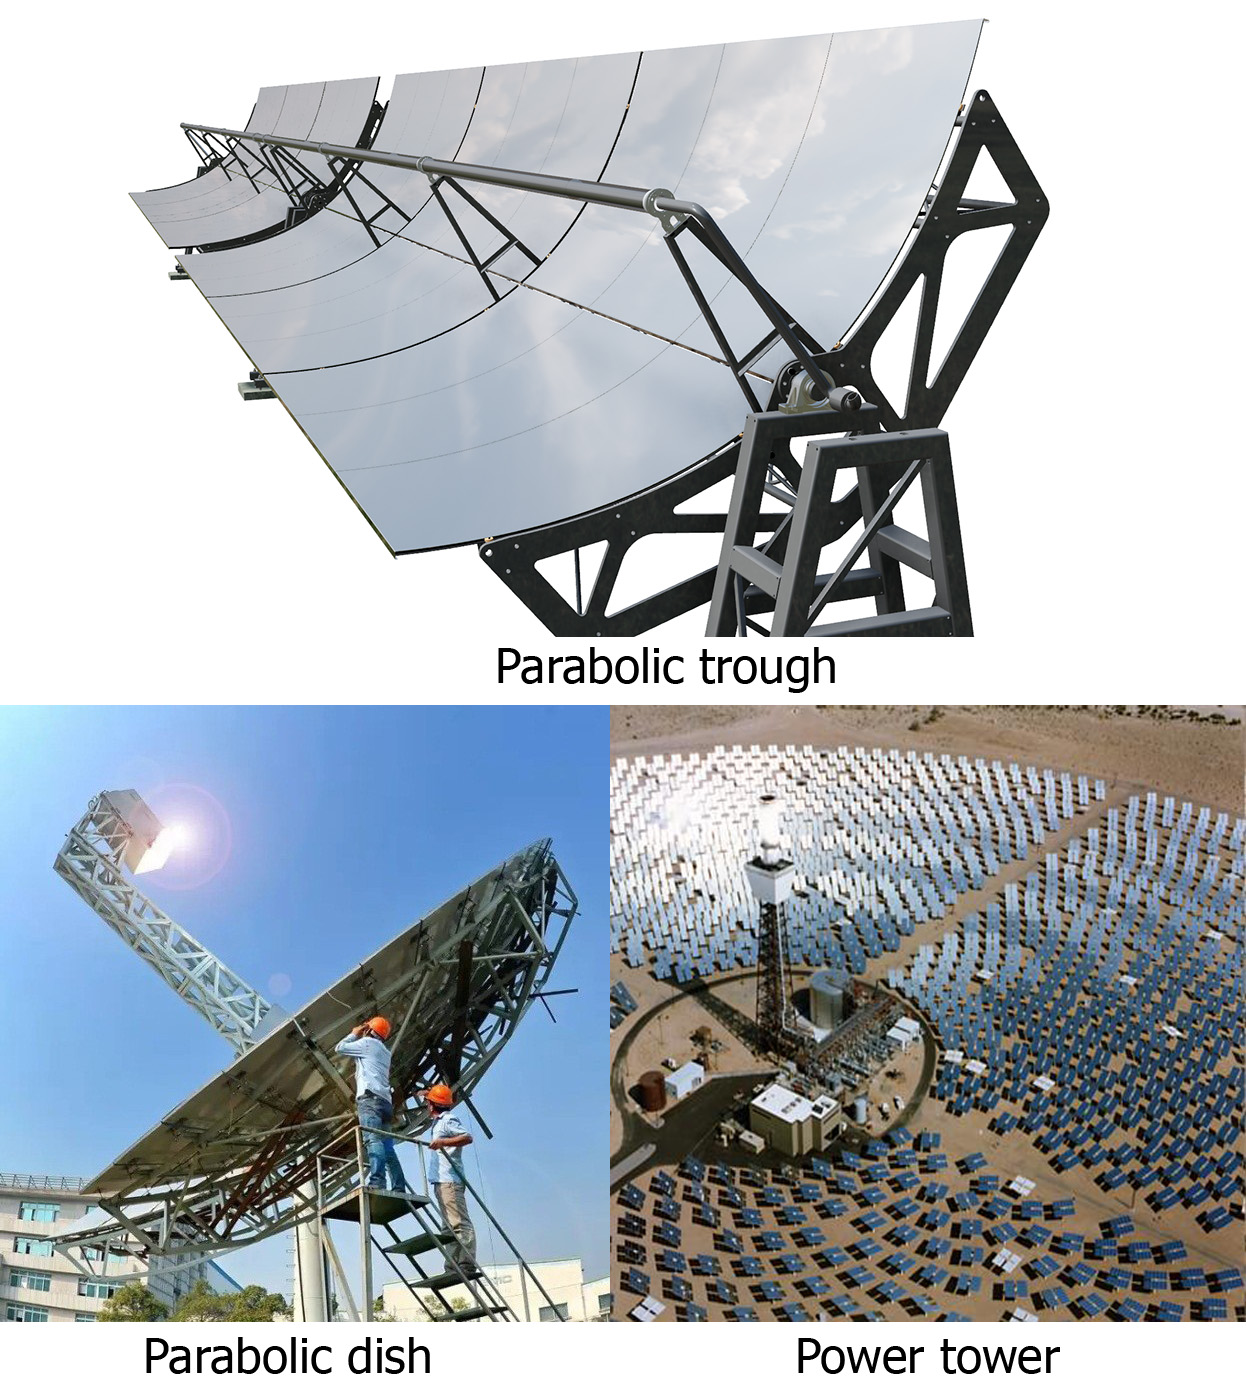
\includegraphics[width=.8\textwidth]{fig/Collectors}
\caption{Examples of the three types of CSP technologies}\label{fig:collectors}
\end{figure}

A parabolic trough is a type of solar thermal collector whose mirror type is straight in one dimension and curved as a parabola in the other two. The reflector follows the sun during the daylight hours by tracking along a single axis. The energy of sunlight is reflected by the mirror and focused on the pipe positioned at the focal line. HTF (e.g. synthetic oil) runs through the pipe to absorb the heat generated by the focused sunlight, then used as the heat source for power generation or heating process.

A parabolic dish is a type of solar thermal collector whose mirror type is part of a circular paraboloid, which can converge the incoming sunlight traveling along the axis to the focus. Two-axis tracking system keeps it always directly towards the sun without cosine loss. It can obtain high concentration ratio and hence high temperature.
Typically, a receiver or a Stirling engine is put at the focal point to absorb the converged energy. 
%Figure~\ref{fig:pd} shows a 38 kW prototype Stirling engine product of Xiangtan Electric Manufacturing Group Co., Ltd. (XEMC).
%\begin{figure}[!ht]
%\centering
%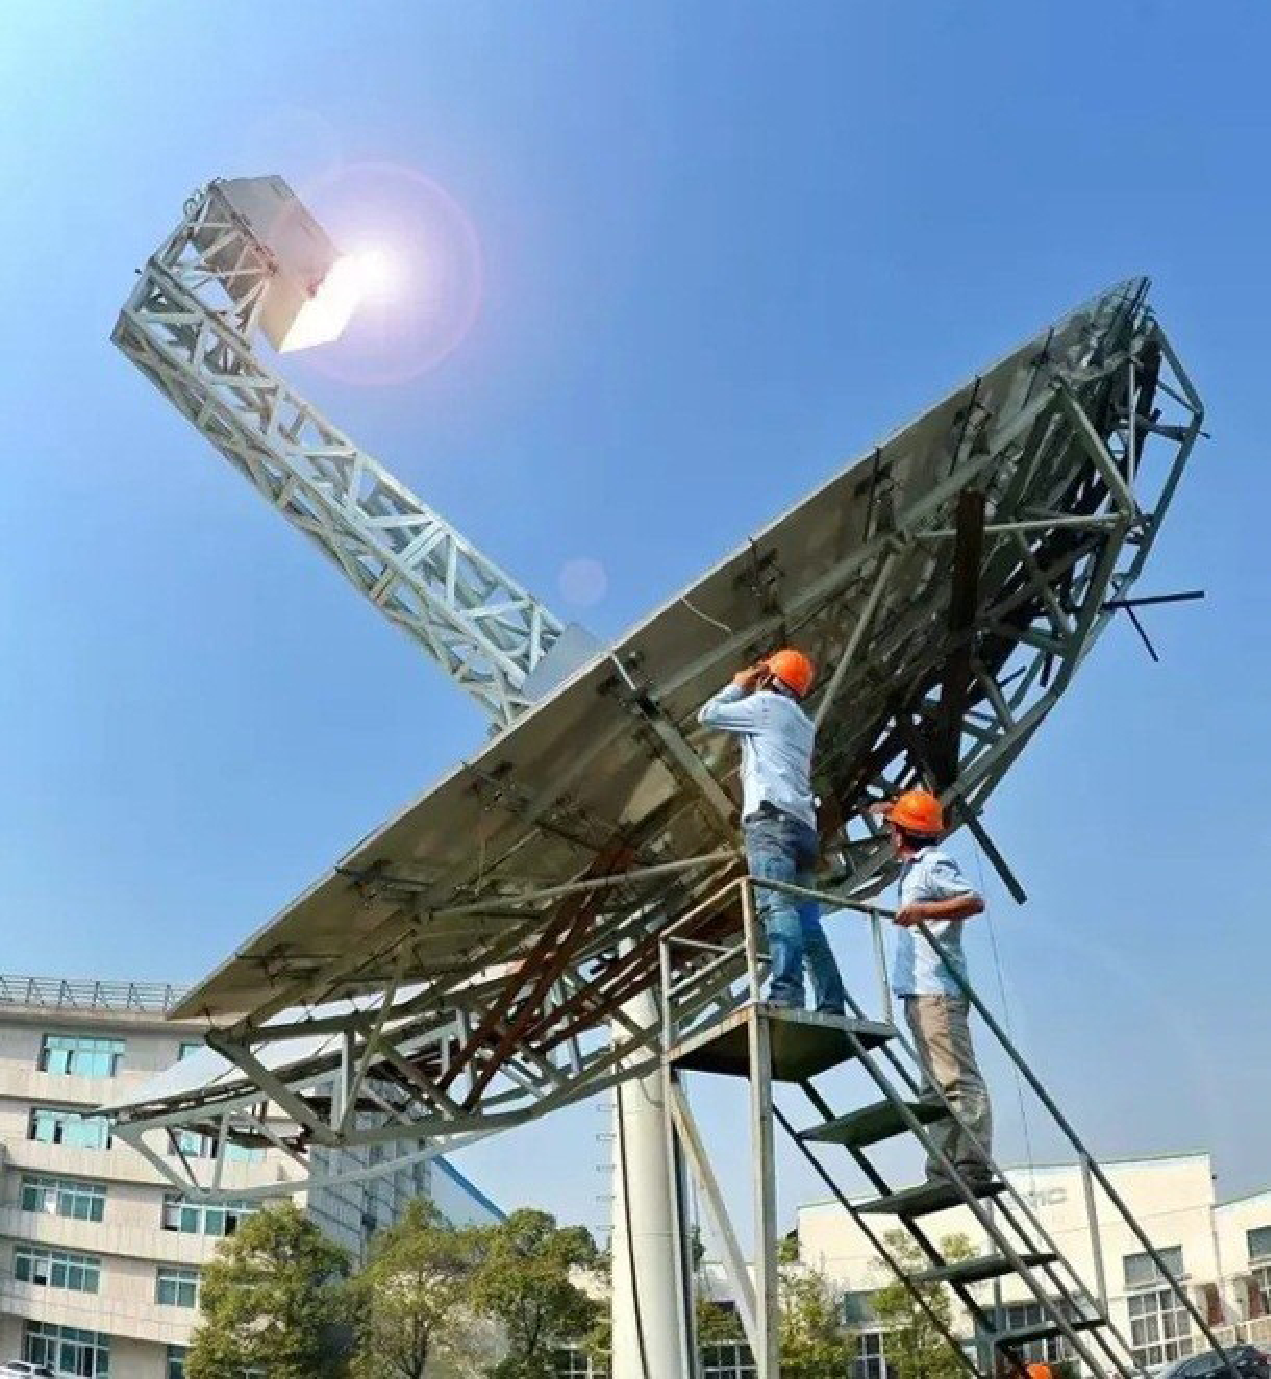
\includegraphics[width=.6\textwidth]{fig/ParabolicDish}
%\caption{A 38 kW prototype Stirling engine product of XEMC}\label{fig:pd}
%\end{figure}

Solar power tower is a type of solar furnace using a tower to receive the focused sunlight. It uses an array of flat, movable mirrors (called heliostats) to focus the sun's rays upon a collector tower. The heliostats track the sun on two axes (east to west and up and down). The receiver absorbs concentrated solar radiation and converts the solar energy into heat. The heat is then transferred to an HTF that carries the heat to a thermodynamic cycle for power generation. 
%Figure~\ref{fig:spt} shows the Solar Two power tower.
%\begin{figure}[!ht]
%\centering
%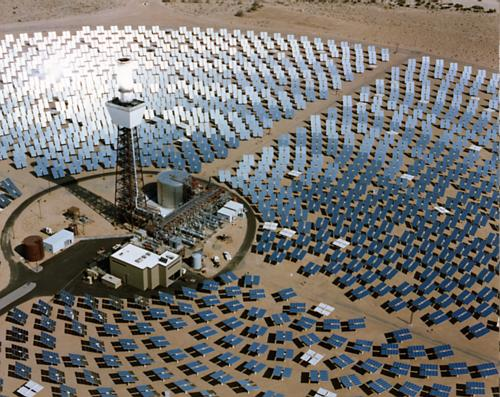
\includegraphics[width=.6\textwidth]{fig/PowerTower}
%\caption{Overall view of Solar Two power tower}\label{fig:spt}
%\end{figure}

%文献2
%In addition to wind and photovoltaic power, concentrating solar thermal power (CSP) will make a major contribution to electricity provision from renewable energies. Drawing on almost 30 years of operational experience in the multi-megawatt range, CSP is now a proven technology with a reliable cost and performance record. In conjunction with thermal energy storage, electricity can be provided according to demand. To date, solar thermal power plants with a total capacity of 1.3 GW are in operation worldwide, with an additional 2.3 GW under construction and 31.7 GW in advanced planning stage. Depending on the concentration factors, temperatures up to 1000°C can be reached to produce saturated or superheated steam for steam turbine cycles or compressed hot gas for gas turbine cycles. The heat rejected from these thermodynamic cycles can be used for sea water desalination, process heat and centralized provision of chilled water. While electricity generation from CSP plants is still more expensive than from wind turbines or photovoltaic panels, its independence from fluctuations and daily variation of wind speed and solar radiation provides it with a higher value. To become competitive with mid-load electricity from conventional power plants within the next 10–15 years, mass production of components, increased plant size and planning/operating experience will be accompanied by technological innovations. On 30 October 2009, a number of major industrial companies joined forces to establish the so-called DESERTEC Industry Initiative, which aims at providing by 2050 15 percent of European electricity from renewable energy sources in North Africa, while at the same time securing energy, water, income and employment for this region. Solar thermal power plants are in the heart of this concept.
% 现有发电技术的优缺点
% 梯级发电的意义

Among the three solar thermal power technologies, parabolic trough is the most mature and commercially deployed technology. However, it has a low concentration ratio, the receiver's temperature is relatively low, the solar-to-electric efficiency is relatively low. Parabolic dish can obtain high temperature thermal energy, its solar-to-electric efficiency is higher than parabolic trough.
Besides, one advantage of parabolic dish is that it requires much less water for power generation. However, solar parabolic dish is not a large-scale application, it's mainly applied for distributed power generation for its compact structure and easy installation. Solar power tower has a very high concentration ratio when more heliostats are used, the receiver's temperature can be very high and it can be applied for large-scale application. However, it has some disadvantages such as high investment and high system complexity. It is currently in rapid development stage.

It is very important to find out a way to utilize the advantages of existing solar thermal power technologies and overcome their disadvantages. In other words, to find out a new technology with higher efficiency and lower cost is urgent.
This research is trying to achieve this by proposing a cascade system that uses different solar collectors and different thermodynamic cycles, which may be a new and feasible technology to realize large-scale, higher efficiency and lower cost solar thermal power generation.

\section{State of the art}
% 范围的大小
%国内外对太阳能光热发电技术的研究现状。
%外文文献-问题-解决方案-本项目需求
Solar thermal power technologies are getting more and more attention. 
Many researchers have done lots of work to research and investigate it to increase its performance or reduce its cost.

\subsection{Parabolic trough}

Parabolic trough solar technology is the most proven and lowest cost large-scale solar power technology available.~\cite{Price2002}

Many of these works have concentrated on experimental work aimed at testing the mechanical and thermal performance of parabolic trough collectors. Dudley et al.~\cite{Dudley1994} tested the collector efficiency and thermal losses of the LS-2 type trough collector. Burkholder and Kutscher~\cite{Burkholder2009} tested the heat losses of Solel's UVAC3 and Schott's 2008 PTR70 parabolic trough collectors. A correlation to estimate the thermal efficiency of the collectors as a function of the absorber temperature was developed. Reddy et al.~\cite{Reddy2015b} developed and investigated six different receiver configurations of trough collectors for performance comparison. Experimental tests were carried out for a 15$\,\mathrm{m^2}$ collector according to ASHRAE 93-1986 test procedure.
Li et al.~\cite{Li2015} carried out experiments to verify the feasibility of proposed end loss compensation methods. A fan-shaped plane mirror was put at one end of the trough collectors to compensate the end loss effect. Results prove that the compensation methods are feasible and effective.
It is well known that experimental studies are the most accurate and convincing method for parabolic trough collector research. However, this method is not only investment required and also time consuming. In order to reduce the R\&D cost and time, parabolic trough collectors are usually modeled.

% 光学效率
Some researchers investigated the optical model of the parabolic trough solar collectors.
Wang et al.~\cite{Wang2016} proposed a mathematical model for optical efficiency of the trough collector and selected three typical regions of solar thermal utilization in China for the model. The model is validated by comparing the test results in parabolic trough power plant, with relative error range of 1\% to about 5\%.
Zou et al.~\cite{Zou2017} investigated the influences of sunshape and incident angle on the optical performance of the trough collectors. It is found that the sunshape has significant effect on the optical efficiency and should be token into consideration in practice. Larger aperture with smaller absorber diameter leads to more end loss caused by incident angle. It is also found that optimal focal length exists for the optical efficiency.
L\"upfert et al.~\cite{Lupfert2006} introduced the specific techniques to analyze the geometry and optical properties of trough collectors and summarized results in collector shape measurement, flux measurement, ray tracing, and thermal performance analysis for parabolic troughs. It is shown that the measurement methods and the parameter analysis give consistent results, which can provide references for the next generation trough collector relevant improvements.
Xu et al.~\cite{Xu2014} analyzed the optical efficiency of a PTC with horizontal north-south axis and proposed a method to compensate the end loss effect of the PTC. The calculation formula of the optical end loss rate and the increased optical efficiency for the system using the compensation method were derived. A five-meter experimental system was built to verify the feasibility of the compensation method proposed. The increased thermal efficiency of the experimental system was measured, and it was proved that the proposed compensation method is feasible.
Huang et al.~\cite{Huang2012} proposed an analytical model for optical performance which employed a modified integration algorithm to simulate the performance of trough collectors. The analytical equation of the optical efficiency of each point of the reflector was deduced to obtain the optical efficiency of the system by integration algorithm.

%热效率和㶲效率分析,想要从能量利用的数量和品质上提升槽式集热器的性能。
Some researchers investigated the exergy performance of the parabolic trough collectors.
Padilla et al.~\cite{Padilla2014} performed a comprehensive exergy balance of a parabolic trough collector based on the previous heat transfer model~\cite{Padilla2011}. The results shown that inlet temperature of heat transfer fluid, solar irradiance, and vacuum in annulus have a significant effect on the thermal and exergetic performance, but the effect of wind speed and mass flow rate of heat transfer fluid is negligible. It was obtained that inlet temperature of heat transfer fluid cannot be optimized to achieve simultaneously maximum thermal and exergetic efficiency because they exhibit opposite trends. Finally, it was found that the highest exergy destruction is due to the heat transfer between the sun and the absorber while for exergy losses is due to optical error.
%Al-Sulaiman~\cite{AlSulaiman2014} presented the exergy analysis of selected thermal power systems driven by PTSCs. The power pf the thermal power system is produced using either a steam Rankine cycle (SRC) or a combined cycle, in which the SRC is the topping cycle and an organic Rankine cycle (ORC) is the bottoming cycle.
Guo et al.~\cite{JiangfengGuo2016-1} investigated the energy efficiency and exergy efficiency of the parabolic trough collector. The result shown that there exists an optimal mass flow rate of working fluid for exergy efficiency, and the thermal efficiency and exergy efficiency have opposite changing tendencies under some conditions.

%热效率模型
Some researchers are dedicated to developing more accurate models using new methods. Behar et al.~\cite{Behar2015} developed and validated a novel parabolic trough solar collector model. The model has been compared with models made by Lab. SNL and NREL. The proposed model has a better accuracy of thermal performance prediction.
% 算法及优化方法
% 光热模型,建模及运算方法
Padilla et al.~\cite{Padilla2011} performed a detailed one dimensional numerical heat transfer analysis of a PTC (Parabolic Trough Collector). To solve the mathematical model of heat transfer of the PTC model, the partial differential equations were discretized and the nonlinear algebraic equations were solved simultaneously. The numerical results was validated to the data from Sandia National Laboratory (SNL).
Hachicha et al.~\cite{Hachicha2013} presented a detailed numerical heat transfer model based on the finite volume method for the parabolic trough collector.  This model is based on finite volume method and ray trace techniques and takes into account the size of the Sun.  The model is thoroughly validated with results from the literature and it shows a good agreement with experimental and analytical results.
Guo and Huai~\cite{JiangfengGuo2016-2} implemented a multi-parameter optimization of parabolic trough solar receiver based on genetic algorithm where Exergy and thermal efficiencies were employed as objective function.
Boukelia et al.~\cite{Boukelia2016} investigated the feed-forward back-propagation learning algorithm with three different variants; Levenberge Marguardt (LM), Scaled Conjugate Gradient (SCG), and Pola-Ribiere Conjugate Gradient (PCG), used in artificial neural network (ANN) to find the best approach for prediction and techno-economic optimization of parabolic trough solar thermal power plant integrated with fuel backup system and thermal energy storage.
Liu et al.~\cite{Liu2012} developed a mathematical model of PTC using the least squares support vector machine (LSSVM) method. Numerical simulations were implemented to evaluate the feasibility and efficiency of the LSSVM method, where the sample data derived from the experiment and the simulation results of two solar collector systems with 30 m$^2$ and 600 m$^2$ solar fields, and the complicated relationship between the solar collector efficiency and the solar flux, the flow rate and the inlet temperature of the heat transfer fluid (HTF) is extracted.
Lobon et al.~\cite{Lobon2014} introduced a computational fluid dynamic simulation approach to predict the behavior of a solar steam generating system, which is located at the Plataforma Solar de Almeria, Spain. The CFD package STAR-CCM+ code has been used to implement an efficient multiphase model capable of simulating the dynamics of the multiphase fluid in parabolic-trough solar collectors. Numerical and experimental data are compared in a wide range of working conditions.
To understand the thermal performance of the collector and identify the heat losses, Mohamad et al.~\cite{Mohamad2014} analyzed the temperature variation of the working fluid, tube and glass along the collector. It is found that using double glazing cover enhances the thermal efficiency of the collector operating at high temperature. However, when the collector length is 10$\,\mathrm{m}$ or less, it is more economical to use a single glass cover for the collector than a double glazing cover.
Also, it is clearly shown that increasing the diameter of absorbing tube enhances the rate of heat transfer losses, consequently decreasing the thermal efficiency of the collector.
Guo et al.~\cite{SuGuo2016} developed a nonlinear distribution parameter model to model the dynamic behaviors of direct steam generation parabolic trough collector loops under either full or partial solar irradiance disturbance.

% 其它用法
Some researchers have proposed some new types of solar trough systems.
Ashouri et al.~\cite{Ashouri2015} coupled a small scale parabolic trough collector and a thermal storage tank along with an auxiliary heater to a Kalina cycle to study the performance of the system throughout the year, both thermodynamically and economically.
% 空气介质
Bader et al.~\cite{Bader2015} developed a numerical model of a tubular vavity-receiver that uses air as the heat transfer fluid. Four different receiver configurations are considered, with smooth or V-corrugated absorber tube and single- or double-glazed aperture window. The different types of energy loss by the collector have been quantified, and the temperature distribution inside the receiver has been studied. The pumping power required to pump the HTF through the receiver has been determined for a 200$\,\mathrm{m}$ long collector row.
Good et al.~\cite{Good2015} proposed solar trough concentrators using air as heat transfer fluid at operating temperatures exceeding 600$\mathrm{^\circ C}$. It consists of an array of helically coiled absorber tubes contained side-by-side within an insulated groove having a rectangular windowed opening. Secondary concentrating optics are incorporated to boost the geometric concentration ratio to 97$\times$.
% 强化换热
Kaloudis et al.~\cite{Kaloudis2016} investigated a PTC system with nanofluid as the HTF in terms of Computational Fluid Dynamics (CFD). Syltherm 800 liquid oil was used as the HTF, and Al$_2$O$_3$ nanoparticles with the concentrations ranges from 0\% to 4\% was investigated. A boost up to 10\% on the collector efficiency was reported for Al$_2$O$_3$ concentration of 4\%.
% 新颖的系统
%Tan et al.~\cite{Tan2014} proposed a two-stage photovoltaic thermal system based on solar trough concentration, in which the metal cavity heating stage is added on the basis of the PV/T stage, and thermal energy with higher temperature is output while electric energy is output. The experimental platform of the two-stage photovoltaic thermal system was established, with a 1.8 m$^2$ mirror PV/T stage and a 15 m$^2$ mirror heating stage, or a 1.8 m$^2$ mirror PV/T stage and a 30 m$^2$ mirror heating stage. The results show that with single cycle, the long metal cavity heating stage would bring lower thermal efficiency, but temperature rise of the working medium is higher, up to 12.06$\mathrm{^\circ C}$ with only single cycle. With 30 min closed multiple cycles, the temperature of the working medium in the water tank was 62.8$\mathrm{^\circ C}$, with an increase of 28.7$\mathrm{^\circ C}$, and thermal energy with higher temperature could be output.
Al-Sulaiman et al.~\cite{AlSulaiman2012} proposed a novel system based on PTC and ORC for combined cooling, heating and power (CCHP). Performance assessment, including efficiency, net electrical power, and electrical to heating and cooling ratios, of the system shown that when CCHP is used, the efficiency increases significantly. This study reveals that the maximum electrical efficiency for the solar mode is 15\%, for the solar and storage mode is 7\%, and for the storage mode is 6.5\%. The maximum CCHP efficiency for the solar mode is 94\%, for the solar and storage mode is 47\%, and for the storage mode is 42\%.
\nomenclature[C]{CCHP}{Combined cooling, heating and power}
\nomenclature[C]{HTF}{Heat Transfer Fluid}
\nomenclature[C]{CFD}{Computational fluid dynamics}
\nomenclature[C]{DSG}{Direct Steam Generation}
\nomenclature[C]{LM}{Levenberge Marguardt}
\nomenclature[C]{SCG}{Scaled Conjugate Gradient}
\nomenclature[C]{PCG}{Pola-Ribiere Conjugate Gradient}
\nomenclature[C]{ANN}{Artificial neural network}
%\nomenclature[C]{PTSTPP}{Parabolic Trough Solar Thermal Power Plant}
\nomenclature[C]{SRC}{Steam Rankine Cycle}
\nomenclature[C]{ORC}{Organic Rankine Cycle}
\nomenclature[C]{PTC}{Parabolic Trough Collector}
\nomenclature[C]{SNL}{Sandia National Laboratory}
\nomenclature[C]{LSSVM}{Least squares support vector machine}

\subsection{Parabolic dish}
\label{sec:pd}

The solar parabolic dish system is known for its highest efficiency of all solar technologies (around 30\%). It is suitable for distributed power generation for its compact structure and easy installation.  

Many researchers conducted experiments to investigate the solar parabolic dish system or to validate proposed models.
To investigate the heat loss of semi-spherical cavity receiver applied for solar parabolic dish system, Tan et al.~\cite{Tan2014b} conducted experiments with different fluid inlet temperatures, receiver inclination angles and aperture sizes. Correlations of Nusselt number as a function of Grashof number were developed by the experiment results.
Chaudhary et al.~\cite{Chaudhary2013} investigated a solar cooker based on dish collector with phase change thermal (PCM) storage unit. Three cases have been considered for the investigation: ordinary solar cooker, solar cooker with outer surface painted black, and solar cooker with outer surface painted black along with glazing. It was observed that the last case shows the best performance, which can store 32.3\% and 26.8\% more heat for the PCM compared with the first and second cases respectively.
Mawire and Taole~\cite{Mawire2014} investigated the thermal performance of a cylindrical cavity receiver for an SK-14 parabolic dish concentrator. The receiver exergy rates and efficiencies are found to be appreciably smaller than the receiver energy rates and efficiencies. The exergy factor is found to be high under conditions of high solar radiation and high operating temperatures. An optical efficiency of around 52\% for parabolic dish system is determined under high solar radiation conditions.
Zhu et al.~\cite{Zhu2015} conducted an experimental investigation of a coil type solar dish receiver. The solar irradiance is about 650$\,\mathrm{W/m^2}$, while the concentrated solar flux at the aperture is approximately 1000$\,\mathrm{kW/m^2}$. The energy and exergy performance of the receiver was analyzed and the experimental results show that, at steady state, the energy efficiency is maintained around 80\%, and the exergy efficiency is around 28\%. 
CRTEn developed a solar dish system using four types of absorbers: flat plat, disk, water calorimeter and solar heat exchanger.~\cite{Skouri2013} For the different types of absorbers, experiments were conducted to obtain the mean concentration ratio and both energy and exergy efficiency. Results shown that thermal energy efficiency of the system varies from 40\% to 77\%, the concentrating system reaches an average exergy efficiency of 50\% and a concentration factor around 178.
Thirunavukkarasu et al.~\cite{Thirunavukkarasu2017} carried out an experimental study to investigate the thermal performance of a cavity receiver for a dish concentrator. The overall system efficiency of the solar collector is 69.47\%. The average exergy efficiency of the receiver is found to be 5.88\% with a peak value of 10.35\%.
Pavlovic et al.~\cite{Pavlovic2017} performed the experimental study of a solar dish system. In this system, different working fluids (water, thermal oil and air) were used to validate the numerical models developed in EES (Engineering Equation Solver). It was found that water is the most appropriate working fluid for low-temperature applications, while thermal oil is the most appropriate working fluid for higher-temperature applications.

Some researchers focused on the dish concentrator, many proposed different shapes of concentrators. The perfect concentrator has a parabolic shape, but for some considerations (better production, safer transportation, lest cost and so on), some solar concentrators are composed of multiple spherically shaped mirrors.
A large dish solar concentrator, SG3, which is about 400$\,\mathrm{m^2}$, was designed and demonstrated in Australian National University in 1994 as shown in Figure~\ref{fig:LargeDish}.~\cite{Lovegrove2011} It successfully proved the technical viability of a concentrator that is approximately three times bigger than any other produced. 
\begin{figure}[!ht]
\centering
\includegraphics[width=.8\textwidth]{fig/largeDish.jpg}
\caption{The SG3 400$\,\mathrm{m^2}$ dish in Australian National University}\label{fig:LargeDish}
\end{figure}
Berumen et al.~\cite{Berumen2004} developed a refector consists of 12 facets made of fiberglass with a reflecting surface made of aluminum sheet with reflectance of 86\%.
Pavlovic et al.~\cite{Pavlovic2014} presented a procedure to design a square facet concentrator for laboratory-scale research on medium-temperature thermal processes. A parabolic collector made up of individual square mirror panels (facets) were investigated. These facets can deliver up to 13.604 kW radiative power over a 250$\,\mathrm{mm}$ radius dish receiver with average concentrating ratio exceeding 1200.
Hijazi et al.~\cite{Hijazi2016} designed a low cost parabolic solar dish concentrator with small-to moderate size for direct electricity generation and special attention is given to the selection of the appropriate dimensions of the reflecting surfaces.
Ma et al.~\cite{Ma2012} designed a solar dish concentrator based on triangular membrane facets. A 600-facet concentrator with focal-diameter ratio of 1.1 will achieve 83.63\% of radiative collection efficiency over a 15$\,\mathrm{cm}$ radius disk located in the focal plane, with a mean solar concentration ratio exceeding 300.
A 3.6-meter diameter stretched-membrane optical facet for a parabolic dish has been successfully designed and demonstrated under contract with Sandia National Laboratories.~\cite{Schertz1991} Twelve facets identical to them will be used to make the lightweight reflector of the dish. The project goal of 2.5$\,\mathrm{mrad}$ surface accuracy was met with each of the two full-sized prototypes, and accuracies of as low as 1.1$\,\mathrm{mrad}$ were achieved.

Many researches investigated the flux distribution and thermal performance of the solar dish receiver.
Shuai et al.~\cite{Shuai2010} developed a flux distribution measurement system for dish concentrators. A charge coupled device camera was applied to obtain the contours of the flux distribution for target placements with different location. Further, the measured flux distributions are compared with a Monte Carlo-predicted distribution. The results can be a valuable reference for the design and assemblage of the solar collector system.
Mao et al.~\cite{Mao2014b} simulated the flux distribution of a dish receiver using MCRT method. The impacts of incident solar irradiation, aspect ratio (the ratio of the receiver height to the receiver diameter), and system error on the radiation flux of the receiver are investigated.
Li et al.~\cite{Li2011b} used the Monte-Carlo ray-tracing method for the radiation flux distribution of the solar dish receiver system. The result was validated by experiment and used as the boundary conditions of a CFD receiver model. The fluid flow and conjugate heat transfer in the receiver was numerically simulated and validated by experiments.
Wang and Laumert~\cite{Wang2017} used the ray-tracing methodology to investigate the effects of cavity surface materials on the flux distribution for an impinging receiver. Five cavity surface materials and their combinations have been studied. The results show that the flux distribution and the total optical efficiency are much more sensitive to the absorptivity on the cylindrical surface than on the bottom.
Blazquez et al.~\cite{Blazquez2016} studied the optimization of the concentrator and receiver cavity geometry of parabolic dish system. Ray-tracing analysis has been performed with the open source software Tonatiuh, a ray-tracing tool specifically oriented to the modeling of solar concentrators.
Reddy et al.~\cite{Reddy2015,Reddy2015b} performed the theoretical thermal performance analysis of a fuzzy focal solar parabolic dish concentrator with modified cavity receiver. Total heat loss from the modified cavity receiver was estimated considering the effects of wind conditions, operating temperature, emissivity of cavity cover and thickness of insulation. Time constant test was carried out to determine the influence of sudden change in solar radiation at steady state conditions. The daily performance tests were conducted for different flow rates.
Vikram and Reddy~\cite{Vikram2015} used a three-dimensional numerical model to investigate the total heat losses of three modified cavity with three configurations for parabolic dish receiver. The effects of cavity diameter ratio, tilt angle, operating temperature, insulation thickness and emissivity on the heat loss of the modified cavity receiver were studied. Based on artificial neural network (ANN) modeling, an improved Nusselt number correlation was proposed for convection, radiation and total heat loss calculation.

Some researchers focused on the solar tracking system.
Patil et al.~\cite{Patil2016} described the development of automatic dual axis solar tracking system for solar parabolic dish. Five light dependent resistors were used to sense the sunlight and two permanent magnet DC motors are used to move the solar dish. A controller software were developed to control the motors using the data sensed by the resistors.
Raturi et al.~\cite{Raturi2014} proposed a solar tracking system based on gravity which does not require any external source of power. The prototype test results and analysis show that the system can run successfully.
Kuang and Zhang~\cite{Kuang2012} developed new design and implementation of tracking system to improve tracking accuracy for dish solar based on embedded system that mixes active and passive tracking.
Jin et al.~\cite{Jin2013} described a two-axis sun tracking system with PLC (programmable logic controller) controlled and a combinative tracking method combined active and passive tracking methods for higher accuracy.
Shanmugam and Christraj~\cite{Shanmugam2005} presented a method of intermittent tracking of the sun in the north-south direction with no tracking in the east-west direction for less energy yield and the frequency of tracking in the north-south direction determined by variations in solar altitude angle and size of the absorber in paraboloidal dish concentrator.
\nomenclature[C]{MCRT}{Monte Carlo Ray Tracing}
\nomenclature[C]{CRTEn}{Research and technologies centre of energy in Borj Cedria}

\subsection{Power tower}
\label{sec:st}

Solar power tower technology is gaining more and more interest for its large scale, high concentration ratio and high operating temperature.
It is widely regarded as the most promising solar thermal power technology.

Advances in the power tower technology are mainly the component update as well as system improvement.
Some researchers focused on the choice of HTF that used in the power tower. 
One already standardized commercial plant cycle is the solar tower with conventional steam cycle.~\cite{Spiros2017} Steam is 
used as both HTF and working fluid in the Rankine cycle. Steam is directly generated in the receiver and flows into the steam turbine for power generation.~\cite{Montes2009,Feldhoff2012,Steinmann2006,Yu2017,Gonzalez2017} Many researchers concerned about using other fluids (molten salt, air) as HTF.
Toto et al.~\cite{Toro2016} proposed an idea of a hybrid power tower using air as the working fluid of a topping Brayton cycle and HTF of a bottoming Rankine cycle.
Rold~\cite{Rold2016} proposed an idea of using supercritical CO$_2$ as HTF. A simplified CFD model has been built to analyze the feasibility of supercritical CO$_2$ as HTF in solar towers. It was found that it is a promising alternative for both better operating conditions and lower maintenance cost.
Joshi et al.~\cite{Joshi2016} used the dynamic simulation technology to evaluate a molten salt central receiver design and control strategies.

Many researchers concerned about the heliostats to reach high tracking accuracies under wind loads and thermal stress situations. On the other hand, trade-off between higher land utilization and lower block ratio is also a hot spot.
% 定日镜
Thalange et al.~\cite{Thalange2017} presented the protocol and results of systematic structural analysis of tripod heliostats to reduce the cost and enhance the mechanical behavior.
Besarati and Yogi~\cite{Besarati2014} developed a new and simple method to improve the calculation speed and accuracy for shading and blocking computation of the heliostat field. The Sassi method~\cite{Sassi1983} is used for the shading and blocking efficiency. A 50$\,\mathrm{MWth}$ heliostat field in Dagget, California, USA was used as a case study for the proposed method.
Wei et al.~\cite{Wei2010} proposed a new method for the design of the heliostat field layout for solar tower power plant. Based on the new method, a new code for heliostat field layout design (HFLD) has been developed and a new heliostat field layout for the PS10 plant at the PS10 location has been designed using the new code. Compared with current PS10 layout, the new designed heliostats has the same optical efficiency but with a faster response speed.

Some researchers concerned about the performance of central receiver of power tower.
Kim et al.~\cite{Kim2015} investigated the heat loss of solar central receiver. Numerical simulations using CFD (Computational Fluid Dynamics) with the consideration of four different receiver shapes were carried out to get the influence on convection and radiation heat losses. Different opening ratio between cavity aperture area and receiver aperture area, receiver temperatures, wind velocities and wind directions (head-on and side-on) were considered for the simulations. Results were used to get a simplified correlation model which gets the fraction of convection heat loss. The correlation obtained shows good agreements with the simulation results. The correlation was also validated with experimental data from three central receiver systems (Martin Marietta, Solar One and Solar Two).
Lara et al.~\cite{Lara2016} presented a novel modeling tool for calculation of central receiver concentrated flux distributions. The modeling tool is based on a drift model that includes different geometrical error sources in a rigorous manner and on a simple analytic approximation for the individual flux distribution of a heliostat. 

%Haroun~\cite{El2015} proposed a novel system combines both solar chimney and solar tower. The solar tower receiver was installed at the top of the chimney. Theoretical study of this novel system was conducted. The results shown that the new system generates more power than conventional system with the same parameters of solar irradiance, collector radius, height of chimney, and height of solar tower. The inlet air speed of the chimney is higher than that of the conventional, and it increases with the solar irradiance. Moreover, the results indicated that there exists a optimum ratio of solar tower height to solar chimney height for the maximum overall power.
Some researchers devoted on the simulation of power tower plants.
Franchini et al.~\cite{Franchini2013} developed a computing procedure for solar tower system under both nominal and part load conditions. A Siemens gas turbine product, SGT-800, was applied for the Integrated Solar Combined Cycle (ISCC) as a study case for the solar tower system. The turbine has a dual pressure heat recovery steam generator, which can be used for the Integrated Solar Combined ISCC plant. A model of Solar Rankine Cycle (SRC) driven by power tower was also developed for comparison. A highest solar-to-electric efficiency of 21.8\% can be achieved by the designed ISCC plant. And in all conditions, the global solar energy conversion efficiency of the ISCC is higher than that of the SRC.
Xu et al.~\cite{Xu2011a,Xu2012} created a model of the 1 MW Dahan solar thermal power tower plant using the modular modeling method. The dynamic and static characteristics of the power plant are analyzed based on these models. Response curves of the system state parameters are given for different solar irradiance disturbances. Conclusions in this paper are good references for the design of solar thermal power tower plant.
Benammar et al.~\cite{Benammar2014} developed a mathematical model based on energy analysis for solar tower power plants. A general nonlinear mathematical model of the studied system  has been presented and solved using numerical optimization methods. The analysis of these results shows the existence of an optimal receiver efficiency value for each steam mass flow, receiver surface temperature and receiver surface area.
\nomenclature[C]{ISCC}{Integrated Solar Combined Cycle}

\subsection{Cascade solar system}
\label{sec:cs}

To fully utilize the features of components of solar thermal power system, cascade solar systems are researched by many researchers. There are mainly two directions of the research of cascade solar systems. One is cascade collection, the other is cascade utilization.

\subsubsection{Cascade collection}

Some researchers have investigated the combination of different types of collectors for CSP to achieve cascade solar collection.
Suzuki~\cite{Suzuki1986} analyzed the solar thermal systems with two different types of collectors connected in series. A value of the collectors, the product of the collector efficiency factor and the optical efficiency,  was revealed to be the key factor to determine whether a cascade system is better than either one of the collectors alone. If the value of the lower concentration ratio collector is lager than that of the higher concentration ratio, the cascade system is more effective. Furthermore, it was found that to obtain the maximum energy gain, there exists the optimum operating conditions.

Kribus et al.~\cite{Kribus1999} proposed an idea of using separate aperture stages for different irradiance distribution. The working fluid is gradually heated when it flow through the receiver elements with increasing irradiance levels. A two-stage system was set up to demonstrate this principle at the Weizmann Institute's Solar Tower. Air was used as the HTF to obtain 750$\mathrm{^\circ C}$ after the low-temperature stage and 1000$\mathrm{^\circ C}$ after the high-temperature stage. Figure~\ref{fig:Kribus1999} shows the two-stage receiver system.
\begin{figure}[!ht]
\centering
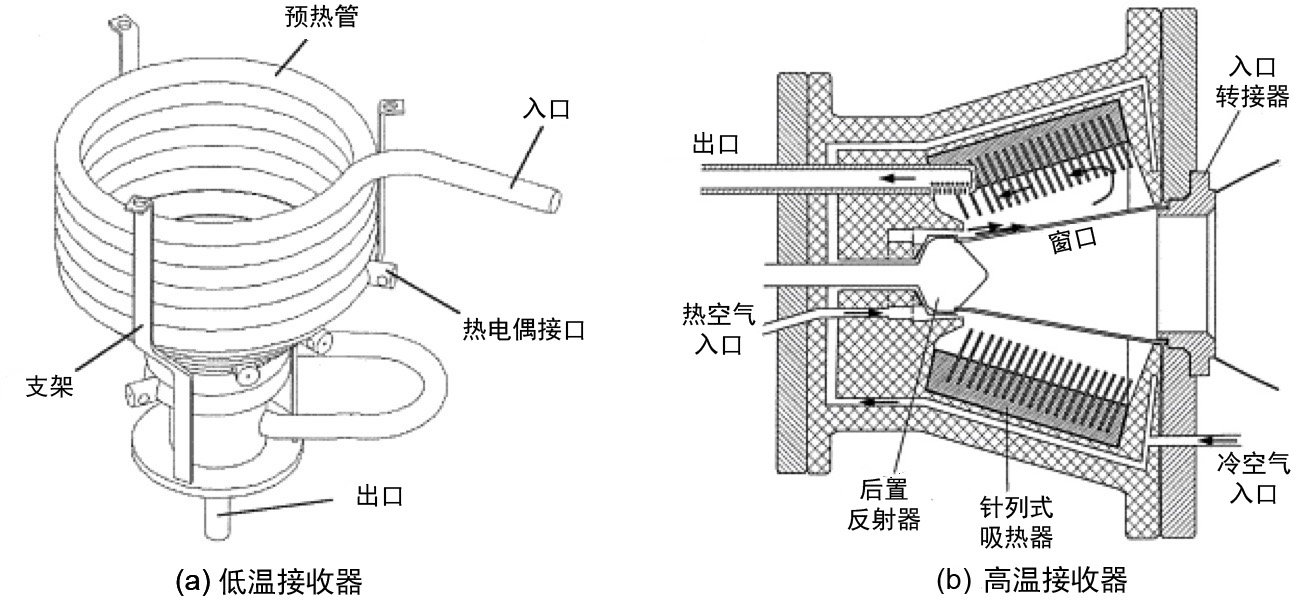
\includegraphics[width=.8\textwidth]{fig/Kribus1999.jpg}
\caption{Two-stage receiver system}
\label{fig:Kribus1999}
\end{figure}

% 组合使用不同厂家的集热器
Gordon and Saltiel~\cite{Gordon1986} presented an analytic method for predicting the long-term performance of solar energy systems with more than one collector brand (``multistage'' systems). This procedure enables the designer to determine the most cost-effective method of combining different collector brands for a given load. The analytic method is illustrated by a solved example which shows that significant savings can be realized by combining different collector brands for a given application (multi-staging).

% Collado2016 and Guallar~\cite{Collado2016} proposed a method breaking the optimization process of solar power tower system down into two consecutive steps.
%    In solar power tower (SPT) systems, selecting the optimum location of thousands of heliostats and the most profitable tower height and receiver size remains a challenge. Given the complexity of the problem, breaking the optimization process down into two consecutive steps is suggested here;
%First, a primary, or energy, optimization, which is practically independent of the cost models, and then a main, or economic, optimization. The primary optimization seeks a heliostat layout supplying the maximum annual incident energy for all the explored combinations of receiver sizes and tower heights. The annual electric output is then calculated as the combination of the incident energy and the simplified (annual averaged) receiver thermal losses and power efficiencies. Finally, the figure of merit of the main optimization is the levelized cost of electric energy (LCOE) where the capital cost models used for the LCOE calculation are reported by the System Advisor Model (SAM)-NREL and Sandia. This structured optimization, splitting energy procedures from economic ones, enables the organization of a rather complex process, and it is not limited to any particular power tower code. Moreover, as the heliostat field layout is already fully optimized before the economic optimization, the profiles of the LCOE versus the receiver radius for the tower heights explored here are sharp enough to establish optima easily. As an example of the new procedure, we present a full thermo-economic optimization for the design of the collector field of an actual SPT system (Gemasolar, 20 MWe, radially staggered surrounding field with 2650 heliostats, 15 h of storage). The optimum design found for Gemasolar is reasonably consistent with the scarce open data. Finally, optimum designs are strongly dependent on the receiver cost, the electricity tariff and the assumed maximum receiver surface temperature.

% 不同集热器型式的对比
%Reddy~\cite{Reddy2009} carried out the numerical analysis of solar dish modified cavity receiver with cone, CPC and Trumpet reflectors is presented. Three-dimensional modeling to estimate the convective and radiative heat loss from the receiver for different angles of inclination and operating temperatures. Incorporating reflectors in the modified cavity receiver for second stage concentration, the natural convection heat losses are reduced by 29.23, 19.81 and 19.16\%, respectively. The receiver with the trumpet reflector has shown better performance as compared to other configurations.

%Mills~\cite{Mills1995}
%
%Maximally concentrating collectors include the class of ideal concentrating collectors, but are a more general class offering many more practical possibilities. By evaluating such configurations using the concept of maximal flux concentration, based upon average radiation flux concentration over the acceptance angle, clear ray trace comparisons may be made between different collector configurations. These comparisons allow the most effective configuration to be selected for a given application. An example of a comparatively simple and practical two-stage concentrator having equal or better maximal performance than previous work for high rim angle primaries is given. This uses an unusual straight section of reflector and allows rays to cross from one reflector segment of the secondary to another. Versions which allow concentration up to 90\% of maximal are described, as are versions achieving 80\% with high collection efficiency. Use of the ~~~ geometrical concentration criterion based upon aperture ratios is suggested to be inappropriate for comparisons.

%空气槽式集热器

%Good et al.~\cite{Good2015} proposed an entirely novel solar receiver design for solar trough concentrators using air as heat transfer fluid at operating temperatures exceeding 600 °C. It consists of an array of helically coiled absorber tubes contained side-by-side within an insulated groove having a rectangular windowed opening. Secondary concentrating optics are incorporated to boost the geometric concentration ratio to 97×. The multiple absorber tubes are connected via two axial pipes serving as feeding and collecting manifolds. The steady-state energy conservation equation coupling radiation, convection, and conduction is formulated and solved numerically using the finite volume technique. The solar flux distribution incident at each absorber tube is determined by Monte Carlo ray-tracing using spectrally and directionally dependent optical properties. Thermal radiative heat exchange is analyzed using the gray-band approximated radiosity method for an enclosure with a selective window. Model validation is accomplished by comparison to on-sun experiments with a 1 m-long solar receiver prototype composed of 7 absorber tubes, mounted on a 4.85 m-aperture solar trough concentrator. Feeding rates in the range of 5–20 ln/min to each absorber tube led to air outlet temperatures of 621–449 °C and a peak receiver efficiency of 64\%.

% 空气碟式系统
% Barder et al.~\cite{Bader2015} developed a numerical model of a tubular cavity-receiver that uses air as the heat transfer fluid using a validated heat transfer model. The receiver is designed for use on a large-span (9 m net concentrator aperture width) solar parabolic trough concentrator. Through the combination of a parabolic primary concentrator with a nonimaging secondary concentrator, the collector reaches a solar concentration ratio of 97.5. Four different receiver configurations are considered, with smooth or V-corrugated absorber tube and single- or double-glazed aperture window. The collector's performance is characterized by its optical efficiency and heat loss. The optical efficiency is determined with the Monte Carlo ray-tracing method. Radiative heat exchange inside the receiver is calculated with the net radiation method. The 2D steady-state energy equation, which couples conductive, convective, and radiative heat transfer, is solved for the solid domains of the receiver cross-section, using finite-volume techniques. Simulations for Sevilla/Spain at the summer solstice at solar noon (direct normal solar irradiance: 847 W$\cdot$m$^{-2}$, solar incidence angle: 13.9$^\circ$) yield collector efficiencies between 60\% and 65\% at a heat transfer fluid temperature of 125$\mathrm{^\circ C}$ and between 37\% and 42\% at 500$\mathrm{^\circ C}$, depending on the receiver configuration. The optical losses amount to more than 30\% of the incident solar radiation and constitute the largest source of energy loss. For a 200 m long collector module operated between 300 and 500$\mathrm{^\circ C}$, the isentropic pumping power required to pump the HTF through the receiver is between 11 and 17 kW.

%多种集热器的混合利用


%Cau~\cite{Cau2014} reported a comparative performance analysis of CSP plants using both parabolic trough and linear Fresnel collectors. A two-tank direct thermal storage system are included and in the Rankine cycle, regenerator, $4\sim6$ steam extractions and air-cooler condenser are used.
Oshida and Suzuki~\cite{Oshida1987} presented the idea of optical cascade heat collection of solar energy. Two absorbers, one warm and the other hot, are used in the cascade system. The warm absorber is heated by the Fresnel lenses and the hot absorber is heated by CPC. HTF flows into the warm absorber firstly and then flows into the hot absorber. The temperature of HTF can increase more effectively by the cascade heating design.

Desai et al.~\cite{Desai2015} presented an integrated CSP plant configuration with the combination of both PTC and LFC. Thermo-economic comparisons between PTC-based, LFC-based and integrated CSP plant configurations, without hybridization and storage, were analyzed. Figure~\ref{fig:Desai2015} shows a simplified schematic of a proposed integrated CSP plant configuration. It is demonstrated that the cost of energy of an integrated CSP plant is 9.6\% cheaper than PTC-based CSP plant and 13.5\% cheaper than LFC-based CSP plant.

Coco et al.~\cite{Coco2015} developed four different line-focusing solar power plant configurations integrated both direct steam generation and Brayton power cycle. In these configurations, collectors are divided into different solar fields to supply different heat demands. This provides the ability to use different types of collectors (parabolic trough and linear Fresnel) in the systems.

\begin{figure}[!ht]
\centering
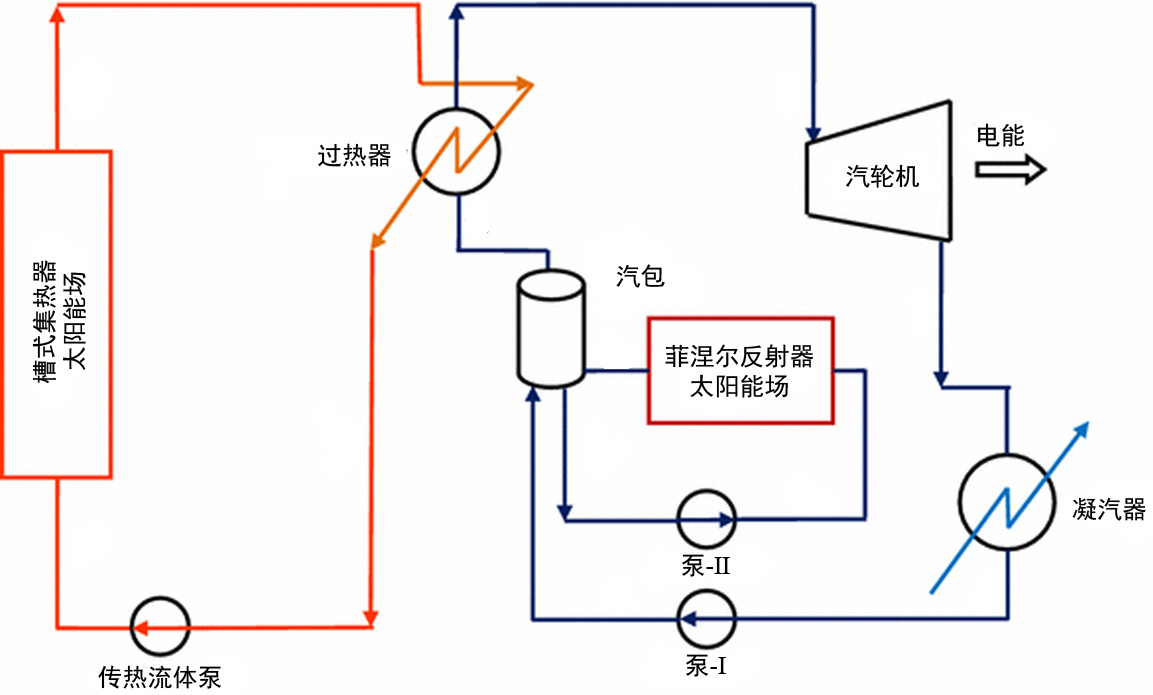
\includegraphics[width=.7\textwidth]{fig/Desai2015.jpg}
\caption{Simplified schematic of a proposed integrated CSP plant configuration}\label{fig:Desai2015}
\end{figure}

\nomenclature[C]{CPC}{Compound parabolic collector}

\subsubsection{Cascade utilization}
%利用槽式集热器为塔式电站的给水预热
%朗肯循环、斯特林循环综合利用
%多级朗肯循环

Many researchers have done the work on the combination of different thermodynamic cycles for CSP. 
Lots of the work focused on integrated solar combined cycle (ISCC) with parabolic trough, where Rankine cycle is used as the bottom cycle.

Li and Yang~\cite{Li2014} proposed a novel two-stage ISCC system that could reach up to 30\% of the net solar-to-electricity efficiency as shown in Figure~\ref{fig:Li2014}. In their research, the impact on the system overall efficiencies of how and where solar energy is input into ISCC system was investigated.
\begin{figure}[!ht]
\centering
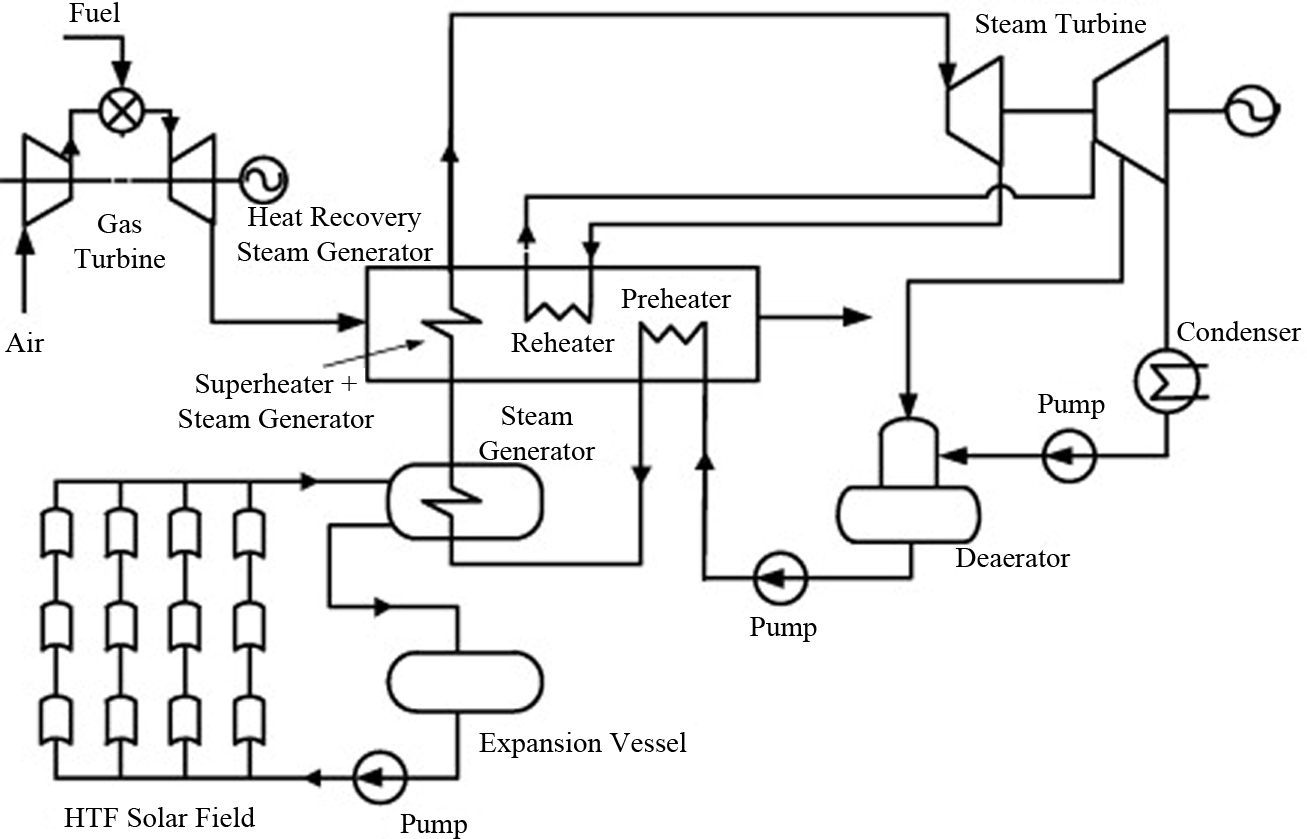
\includegraphics[width=.8\textwidth]{fig/Li2014.jpg}
\caption{The proposed ISCC scheme}\label{fig:Li2014}
\end{figure}

Gulen ~\cite{Gulen2015} used the exergy concept of the second law of thermodynamics to simplify the optimization process of ISCCS. After the exergy analysis, physics-based, user-friendly guidelines were provided for ISCC designs.

Shaaban ~\cite{Shaaban2016} introduced a novel ISCC with steam and organic Rankine cycles. The ORC was used in order to intercool the compressed air and produce a net power from the received thermal energy. The proposed cycle performance was studied and optimized with different ORC working fluids. Figure~\ref{fig:Shaaban2016} shows the schematic of the proposed ISCC.
\begin{figure}[!ht]
\centering
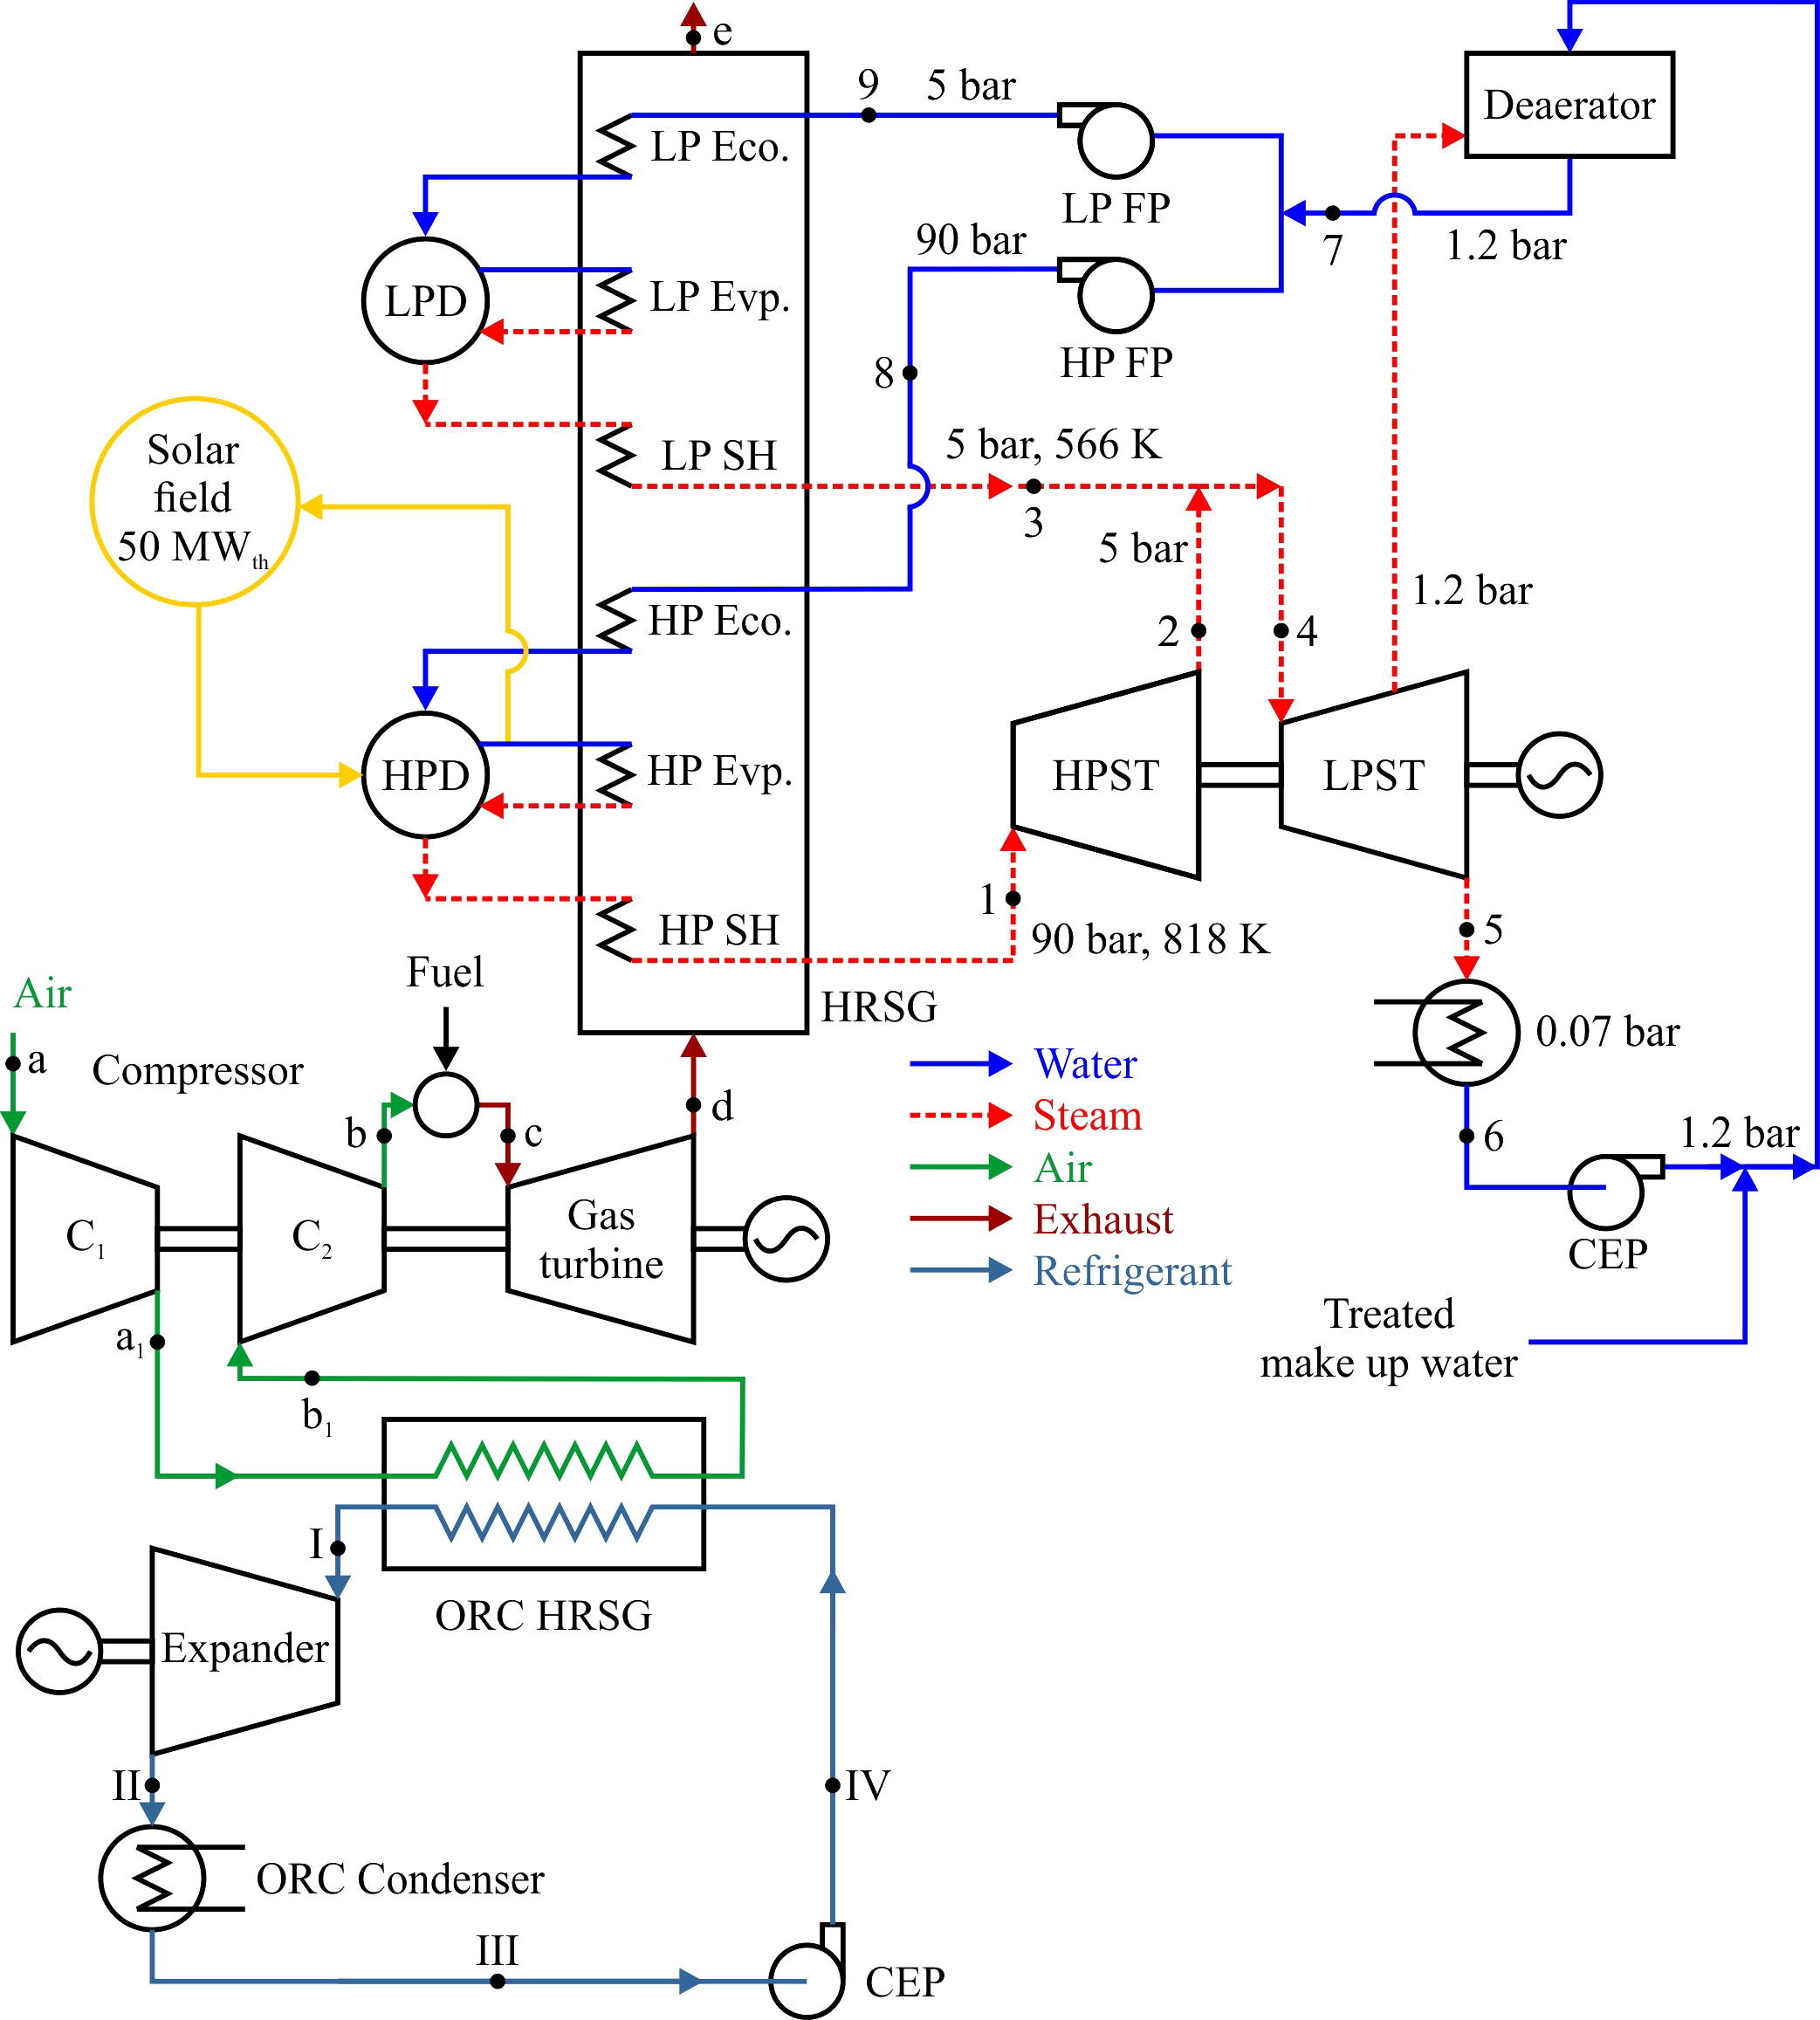
\includegraphics[width=.8\textwidth]{fig/Shaaban2016.jpg}
\caption{Schematic of the proposed ISCC with two bottoming cycles}\label{fig:Shaaban2016}
\end{figure}

Alqahtani and Dalia~\cite{Alqahtani2016} quantified the economic and environmental benefits of an ISCC power plant relative to a stand-alone CSP with energy storage, and a natural gas-fired combined cycle plant. Results show that integrating the CSP into an ISCC reduces the LCOE of solar-generated electricity by 35-40\% relative to a stand-alone CSP plant, and provides the additional benefit of dispatch ability.

Manente~\cite{Manente2016} developed a 390$\,\mathrm{MWe}$ three pressure level natural gas combined cycle to evaluate different integration schemes of ISCC. Both power boosting and fuel saving operation strategies were analyzed in the search for the highest annual efficiency and solar share. Result shown that, compared to power boosting, the fuel saving strategy shows lower thermal efficiencies of the integrated solar combined cycle due to the efficiency drop of gas turbine at reduced loads.
%Rovira et al.~\cite{Rovira2016} compared the annual performance and economic feasibility of ISCC using two solar concentrating technologies: parabolic trough collectors (PTC) and linear Fresnel collectors (LFC). Different configurations were considered and results shown that only evaporative configuration is the most suitable choice.

Turchi et al.~\cite{Turchi2014} represented two new conceptual hybrid designs for ISCC with parabolic trough. In the first design, gas turbine waste heat is supplied for both heat transfer fluid heating and feed water preheating. In the second design, gas turbine waste heat is supplied for a thermal energy storage system.

Mukhopadhyay and Ghosh~\cite{Mukhopadhyay2016} presented a conceptual configuration of a solar power tower combined heat and power plant with a topping air Brayton cycle. The conventional gas turbine combustion chamber is replaced with a solar receiver. A simple downstream Rankine cycle with a heat recovery steam generator and a process heater have been considered for integration with the solar Brayton cycle.

Li et al.~\cite{Li2016a} presented a novel cascade system using both steam Rankine cycle and organic Rankine cycle. Screw expander is employed in the steam Rankine cycle for its good applicability in power conversion with steam-liquid mixture. The heat released by steam condensation is used to drive the organic Rankine cycle.

Al-Sulaiman~\cite{AlSulaiman2014} compared the produced power of an SRC-ORC combined cycle with traditional SRC cycle. The SRC is driven by parabolic trough solar collectors, and the ORC cycle is driven by the condensation heat of the SRC.

Dunham and Lipi~\cite{Dunham2013} proposed a single Brayton and a combined Brayton-Rankine power cycle for distributed solar power generation and compared its theoretical efficiency to a single Brayton cycle. Different working fluids were examined as working fluids in the bottoming Rankine cycle. It is found that the combination of the Brayton topping cycle using carbon dioxide and the Rankine bottoming cycle using R-245fa gives the highest combined cycle efficiency of 21.06\%, while a single Brayton cycle is found to reach a peak cycle efficiency of 15.31\% with carbon dioxide at the same design point conditions. 

Bahrami et al.~\cite{Bahrami2013} proposed a combined ORC power cycle. An ORC was used as the cold-side heat rejector of a Stirling engine. The operating temperatures of the ORC are between 80$\mathrm{^\circ C}$ and 140$\mathrm{^\circ C}$ and the combined system can achieve 4\% to 8\% higher efficiency compared with a standard Stirling cycle.

Thierry et al.~\cite{Thierry2016} proposed a nonlinear optimization formulation of multistage Rankine cycle with two types of configurations. Both cascade style and series style of the ORC are considered. The results show that for some cases the multistage configurations can achieve higher efficiency at low temperature.

Bahari et al.~\cite{Bahari2016} considered the optimization of an integrated system using organic Rankine cycle to utilize the heat released by the Stirling cycle. However, the integrated system is a primitive design and it takes no consideration of the application in CSP.

\nomenclature[C]{LFC}{Linear Fresnel Collector}

\section{Literature summary}
Reviewing the former literatures concerning solar thermal power it can be found that most of the research works have focused on specific solar thermal power technologies to increase efficiency or reduce costs. 

A small number of researchers have also studied the cascade collection or cascade utilization of solar energy. 

There is no literature on the combination of cascade collection and cascade utilization in one cascade solar thermal power system. No systematically analysis of the cascade system has been found.

\section{Research content}
\label{sec:researchContent}
% 改进点,重点,难度
% 技术路线

This research is based on the international cooperation project "Collaborative research on key technologies to produce electricity by cascade utilization solar thermal energy" as the background. The objective of this project is to research the equipment of solar thermal power generation system, to propose, develop and optimize a solar thermal cascade system depending on the advantages and disadvantages of the solar thermal power generation systems, and to explore a new feasible technology for large-scale solar thermal power generation. The main research contents of this thesis are as follows:

\begin{enumerate}[label=(\arabic*)]
	
	\item Selecting reasonable topologies for cascade solar thermal power generation systems. According to the thermodynamic characteristics and operating behaviors of components in thermal power generation systems, reasonable topologies are selected. These topologies should be able to embody the benefits of cascade systems and help to improve the performance of solar thermal power system. 

	\item Establishing the mechanical model of each component in solar thermal power generation system. Based on the governing equations and operating characteristics of each component, a mechanism model will be established. Object-oriented features will be applied to create component models easy to combine, extend, and replace.

	\item System modeling for each proposed cascade system scheme. Based on the mechanism models of the components, a software that provides the functions of system topology arrangement, component connection, parameter setting and environment selection will be developed for the system investigation.

	\item Optimizing the subsystem of the cascade system. Specifically, a staged heating method will be analyzed for the optimization of the steam generating system. Different layouts of Stirling engines will be analyzed to find out best layouts of the Stirling engines in the cascade system.

	\item Finding out the conditions conductive for cascade solar thermal power application.  Selecting appropriate stand-alone systems for comparative analysis of the cascade systems. Analysis of the influences of various parameters on the efficiency difference between cascade system and its corresponding stand-alone systems will be conducted.

	\item Building a solar thermal power generation test platform to carry out experimental works for solar thermal power generation. Special experiment cases considering the features of solar irradiance need to be designed to investigate the impact of different factors on the system performance. Influences of different factors on the performance of components will be investigated. Thermal performances of trough collectors and dish collectors will be analyzed, and the simulation models will be validated.
\end{enumerate}